
\subsection{Small Boat Fleet and Carbon Emissions}
Previous work related to estimating small-scale vessels without machine learning methods includes using top-down and bottom-up approaches and the use of statistical assumptions. 

Parker et al.~\cite{parker2018fuel} used a top-down approach to estimate fishing sector emissions in 2011, which reached about 179 Mt \ch{CO2e}, representing 17.1\% of the total large fishing ship emissions in that year~\cite{smith2015third}. However, their work only distinguished between motorised and non-motorised fishing vessels. Greer et al.~\cite{GREER2019103382} took a bottom-up approach to classify the fishing fleet in six different sizes, three below 25 metres long. The findings show that the small fishing boat fleet in 2016 emitted 47 Mt \ch{CO2} about 22.7\% of the total fishing fleet. Ferrer et al.~\cite{ferrer2021mexican} used an activity-based method using GPS, landing and fuel used data to estimate the fishing activity around Baja California Peninsula in Mexico. They found that just the small-scale fishing fleet produced 3.4 Mt of \ch{CO2e} in 2014. To put this into context, Mexico’s national inventory for the shipping sector in 2014 was recorded at just 2.2 Mt \ch{CO2e}, clearly placing into perspective the role of this fleet segment on national inventories~\cite{inecc2020inventario}.

Several authors have proposed using AIS to monitor the carbon emissions of the fleet ~\cite{Traut2013MonitoringSE, Johansson2016ACM, Mabunda2014EstimatingCD, Hensel2020GreenSU, Han2016RealtimeIA}. Johansson et al.~\cite{Johansson2018ModelingOL} proposed a new model (FMI-BEAM) to describe leisure boat fleet emissions in the Baltic Sea region with over 3,000 dock locations, the national small boat registry, AIS data and vessel survey results. However, the method cannot cover countries with no national registry for small boats. Besides, small boats are not just leisure boats. Ug{\'e} et al.~\cite{Ug2020EstimationOW} estimated global ship emissions with the help of data from AIS. They used more than three billion daily AIS data records to create an activity database that captured ship size, speed, and meteorological and marine environmental conditions. This method is highly dependent on AIS data, however, which does not capture the activity of small boats.

Zhang et al. ~\cite{Zhang2019TheSO} included unidentified vessels in the AIS-based vessel emission inventory. In doing so they developed an AIS-instrumented emissions inventory, including both identified and unidentified vessels. In particular, missing vessel parameters for unidentified vessels were estimated from a classification regression of similar vessel types and sizes in the AIS database. However, the authors did not discuss whether the regression model applies to vessels in most coastal areas. Nor did they explore regional vessel diversity in the database, so statistical inferences and levels of uncertainty about the applicability of their method to other unidentified vessels in a defined single region (e.g. small boats in the Gulf of California, Mexico) cannot be made.

\subsection{Convolutional Neural Network Architecture}
\begin{figure*}[!t]
    \centering
    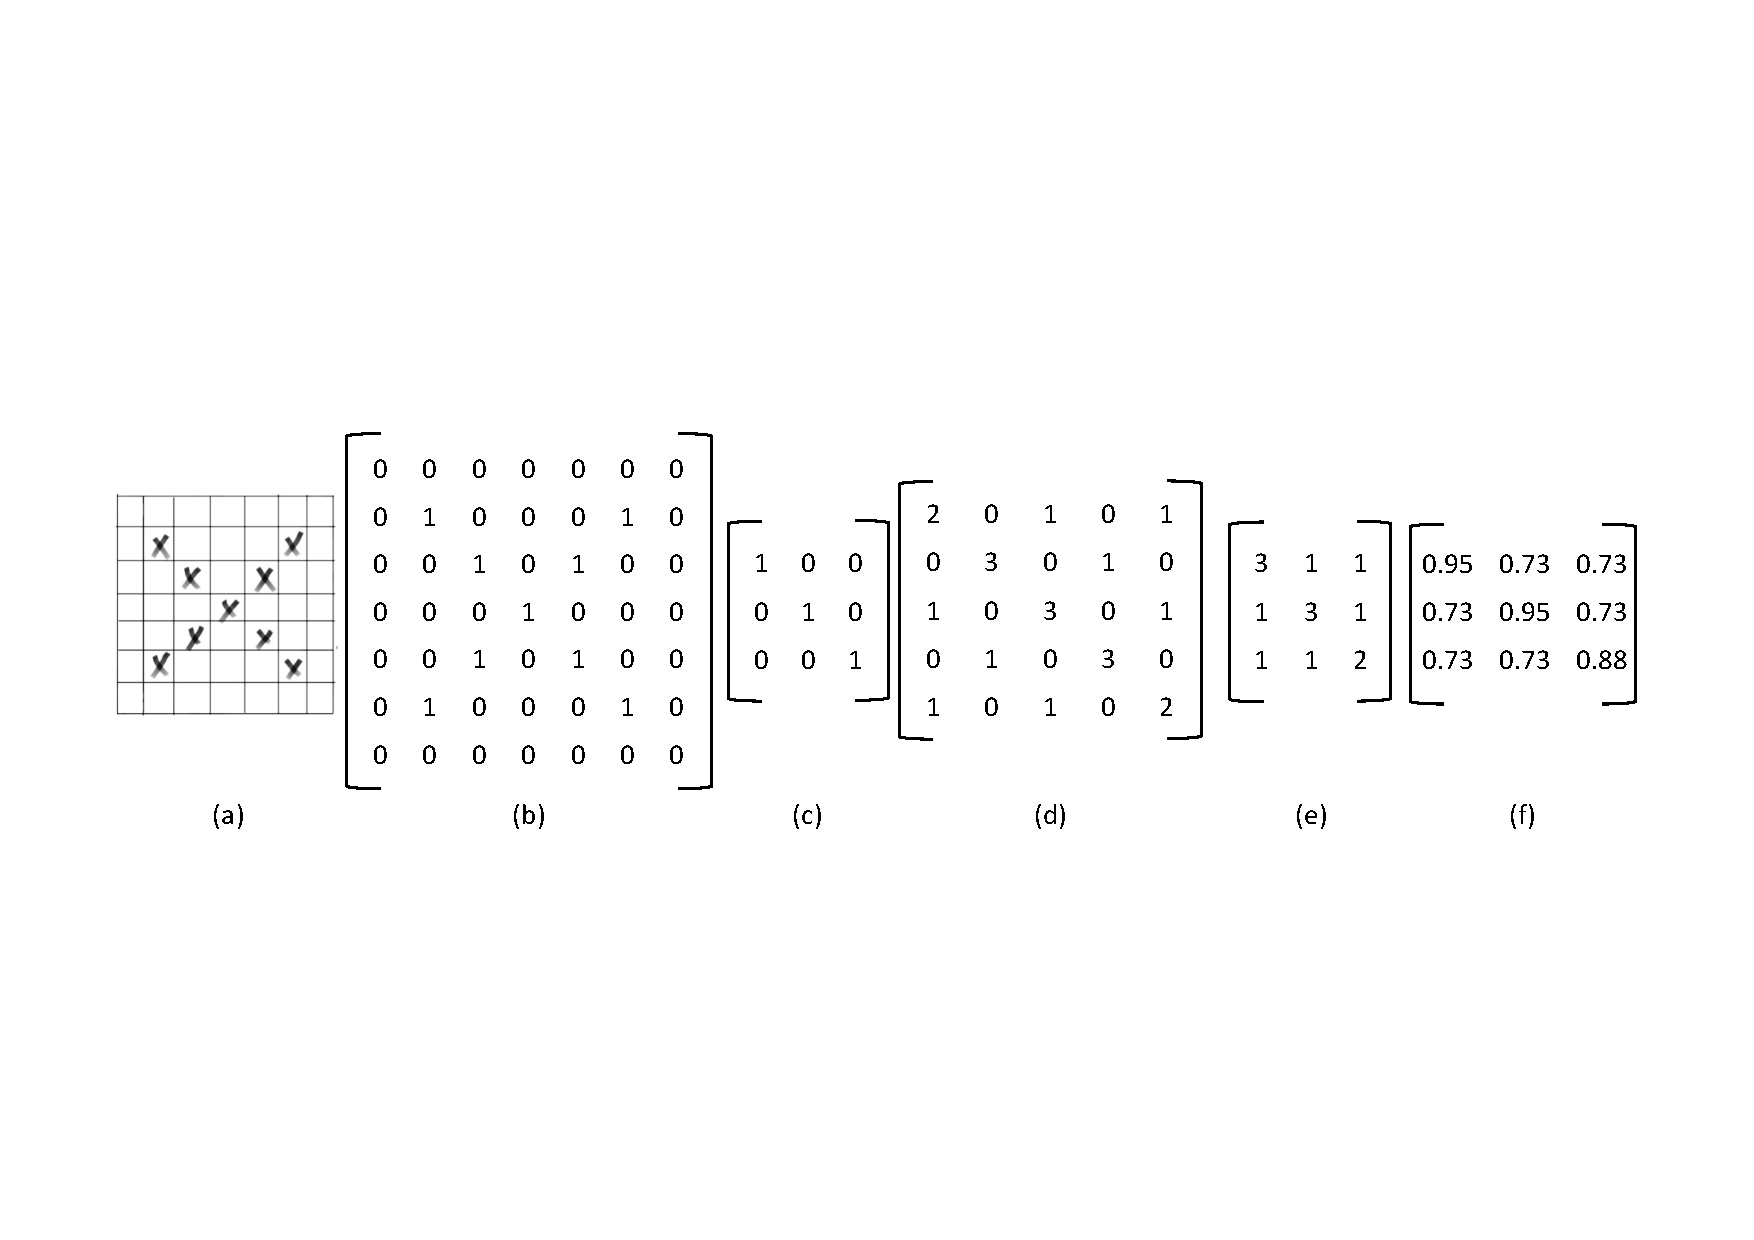
\includegraphics[width=7in]{img/X.pdf}
    \caption{From left to right: (a) Letter X in a 7x7 image; (b) Letter X in a 7x7 matrix; (c) A 3x3 convolution kernel; (d) A 5x5 feature map; (e) A 3x3 feature map after pooling; (f) A 3x3 feature map after activating with sigmoid function.}
    \label{X}
\end{figure*}




Neural networks originate from the human perception of the brain. In 1943, American neuroscientists McCulloch and Pitts proposed a theory that every neuron is a multiple-input single-output structure~\cite{mcculloch1943logical}. Furthermore, there are only two possibilities for this output signal: zero or one, which is very similar to a computer.

In image recognition, a 7x7 image, for example, has 49 elements or cells. If `X' is inputted to the grid, as shown in Figure~\ref{X}a, the computer will interpret it as a series of numbers (e.g. zeros and ones) as seen in Figure~\ref{X}b. If each cell is either black or white, for example, black can be assigned as one while white would be zero, resulting in a 7x7 matrix filled with zeros and ones. After feeding the algorithm as much data as available, it will be trained to find parameters to determine if the object is an `X' or not. For example, if it is a grey-scale picture, each number is neither zero nor new, but rather a grey-scale value from 0 to 255. If it is a colour image, it will use the Red-Green-Blue (RGB) colour range. Essentially, no matter what the image is, it can be interpreted as a combination number inside a matrix, this eventually working as the input of the neural network. The goal of training a neural network is to find the parameters that make the loss function - it measures how far an estimated value is from its true value - smallest. However, the method described above is time-consuming and computationally expensive to train real-world images. Besides, the algorithm will be hard to recognise once the image is dilated, rotated or changed.


Based on the Neocognitron Model of Fukushima~\cite{fukushima1982neocognitron}, LeCun~\cite{lecun1995convolutional} invented a practical method for image recognition, called the convolutional neural network. The role of convolution is to use a mathematical method to extract critical features from the image. This is achieved by extracting the features to use a convolution kernel to carry out the convolution operation. The convolution kernel is a matrix, usually 3x3 or 5x5. For instance, if the convolution kernel is 3x3, see Figure~\ref{X}c, then a convolution operation will be undertaken with the 7x7 "X" matrix (Figure~\ref{X}b) and the kernel (Figure~\ref{X}c). The operation result is also known as a feature map (Figure~\ref{X}d)~\cite{bouvrie2006notes}.


The feature map reinforces the features of the convolution kernel. The 3x3 convolution kernel portrayed in Figure~\ref{X}c) only has three oblique blocks of pixels that are ones. So if the original 7x7 matrix (Figure~\ref{X}b) also has diagonal pixel blocks of ones, the number would be extensive when the convolution operation is complete, which means the desired feature has been extracted. The smaller the value of the pixel block in the other positions of the feature map (Figure~\ref{X}d), the less it satisfies the feature. In general, different convolution kernels make it possible to achieve different feature maps.

The next step after convolution is pooling. The pooling method can reduce the feature map size and maintain similar features to the feature map before the pooling process. Figure~\ref{X}e shows the relatively small feature map after pooling the 5x5 matrix (Figure~\ref{X}d).


The step after pooling is activation. The activation function decides whether the neuron should be activated by computing the weighted sum and further adding the bias. The essence of the activation function is to introduce nonlinear factors to solve problems that a linear model cannot solve~\cite{lin2018research}. For example, after activating the sigmoid function, each element in the feature map would be between 0 and 1, as shown in Figure~\ref{X}f.

It is worth noting that the initial convolution kernel may be artificially set. Nevertheless, machine learning will go backwards to adjust and find the most suitable convolution kernel based on its data. Since an image generally has many features, there will be many corresponding convolution kernels. After many convolutions and poolings, features can be found, including the diagonal lines of the image, the contours, and the colour features. This information is taken and fed into the fully connected network for training, and it is finally possible to determine what the image is.


\subsection{Convolutional Neural Networks in Image Recognition}
\label{sec2.2}
The above literature review has demonstrated that past literature on shipping carbon inventories has not focused on small vessels. Thus the topic of activity-based emission inventories for this segment is an important gap in the literature. There is still considerable work to be done to understand how the small boat fleet operates, what fuels are used, and the level of activity. However, with the development and maturation of a range of computer vision techniques such as convolutional neural networks (CNNs), it may be possible to accurately identify small vessels from open satellite imagery and support understanding of this ship segment. 

One of the computer vision's most fundamental and challenging problems is target detection. The main goal of target detection is to determine the location of an object in an image based on a large number of predefined classes. Deep learning techniques, which have emerged in recent years, are a powerful method for learning features directly from data and have led to significant breakthroughs in the field of target detection. Furthermore, with the rise of self-driving cars and face detection, the need for fast and accurate object detection is growing.

In 2012, AlexNet, a deep convolutional neural network (DCNN) proposed by Krizhevsky et al.~\cite{krizhevsky2012imagenet}, achieved record accuracy in image classification at the ImageNet Large-Scale Visual Recognition Challenge (ILSRVC), making convolutional neural networks the dominant paradigm for image recognition. Next, Girshick et al.~\cite{girshick2014rich} introduced Region-Based Convolutional Neural Networks (R-CNN), the first convolutional neural network (CNN)-based object detection method. The R-CNN algorithm represents a two-step approach in which a region proposal is generated first, and then a CNN is used for recognition and classification. Compared to the traditional sliding convolutional window to determine the possible regions of objects, R-CNN uses selective search to pre-extract some candidate regions that are more likely to object in order to avoid computationally costly classification and object searches, which makes it faster and significantly less computationally expensive~\cite{ uijlings2013selective, girshick2014rich}. Overall, the R-CNN approach is divided into four steps:

\begin{itemize}
    \item Generate candidate regions.
    \item Extract features using CNN on the candidate regions.
    \item Feed the extracted features into a Support Vector Machine (SVM) classifier.
    \item Correct the object positions by using a regressor.
\end{itemize}

However, R-CNN also has drawbacks: the selective search method is slow in generating positive and negative sample candidate regions for the training network, which affects the overall speed of the algorithm; R-CNN needs to perform feature extraction once for each generated candidate region separately; there are a large number of repeated operations which limits the algorithm performance ~\cite{huang2017speed}.

Since its inception, R-CNN has undergone several developments and iterations: Fast R-CNN, Faster R-CNN and Mask R-CNN~\cite{girshick2015fast, ren2015faster, he2017mask}. The improvement of Fast R-CNN is the design of a pooling layer structure for Region of Interest (ROI). The pooling stage effectively solves the R-CNN operation that crops and scales image regions to the same size, speeding up the algorithm. Faster R-CNN replaces the selective search method with Region Proposal Network (RPN) ~\cite{ren2015faster}. The selection and judgment of candidate frames are handed over to the RPN for processing, and candidate regions are subjected to multi-task loss-based classification and localisation processes. 

Several convolutional neural network-based object detection frameworks have recently emerged that can run faster, have a higher detection accuracy, produce cleaner results and are easier to develop. Compared to the Faster RCNN model, the YOLO model can better detect smaller objects, i.e. traffic lights at a distance~\cite{Dwivedi2020YOLOv5}, which is important when detecting objects in satellite images. Also, the YOLO model has a faster end-to-end run time and detection accuracy than the Faster RCNN~\cite{Dwivedi2020YOLOv5}. Mask R-CNN upgrades the ROI Pooling layer of the Fast R-CNN to an ROI align layer and adds a branching FCN layer, the mask layer, to the bounding box recognition for semantic mask recognition~\cite{he2017mask}. Thus, the Mask R-CNN is essentially an Instance Segmentation algorithm, compared to Semantic Segmentation\footnote{In computer vision, image segmentation is the process of partitioning an image into multiple image segments, also known as image regions or image objects.}. Instance Segmentation is a more fine-grained segmentation of similar objects than Semantic Segmentation.

However, even traditional CNNs can be very useful for large-scale image recognition. For example, Simonyan and Zisserman~\cite{Simonyan2015VeryDC} researched the effect of convolutional network depth on its accuracy in large-scale image recognition settings. Their research found that even with small (3x3) convolution filters, significant accuracy is achieved by pushing the depth from 16 to 19 weight layers.

Finally, this study intends to develop the first stages of BoatNet. This image recognition model can detect small boats in any sea area which, in turn and with further development, could significantly reduce uncertainty in the estimation of small boat fleet emission inventories in countries where access to tracking infrastructure, costly satellite databases and labour-intensive methodologies are important barriers.
